\documentclass{standalone}


\usepackage[europeanresistors,americaninductors]{circuitikz}

\begin{document}
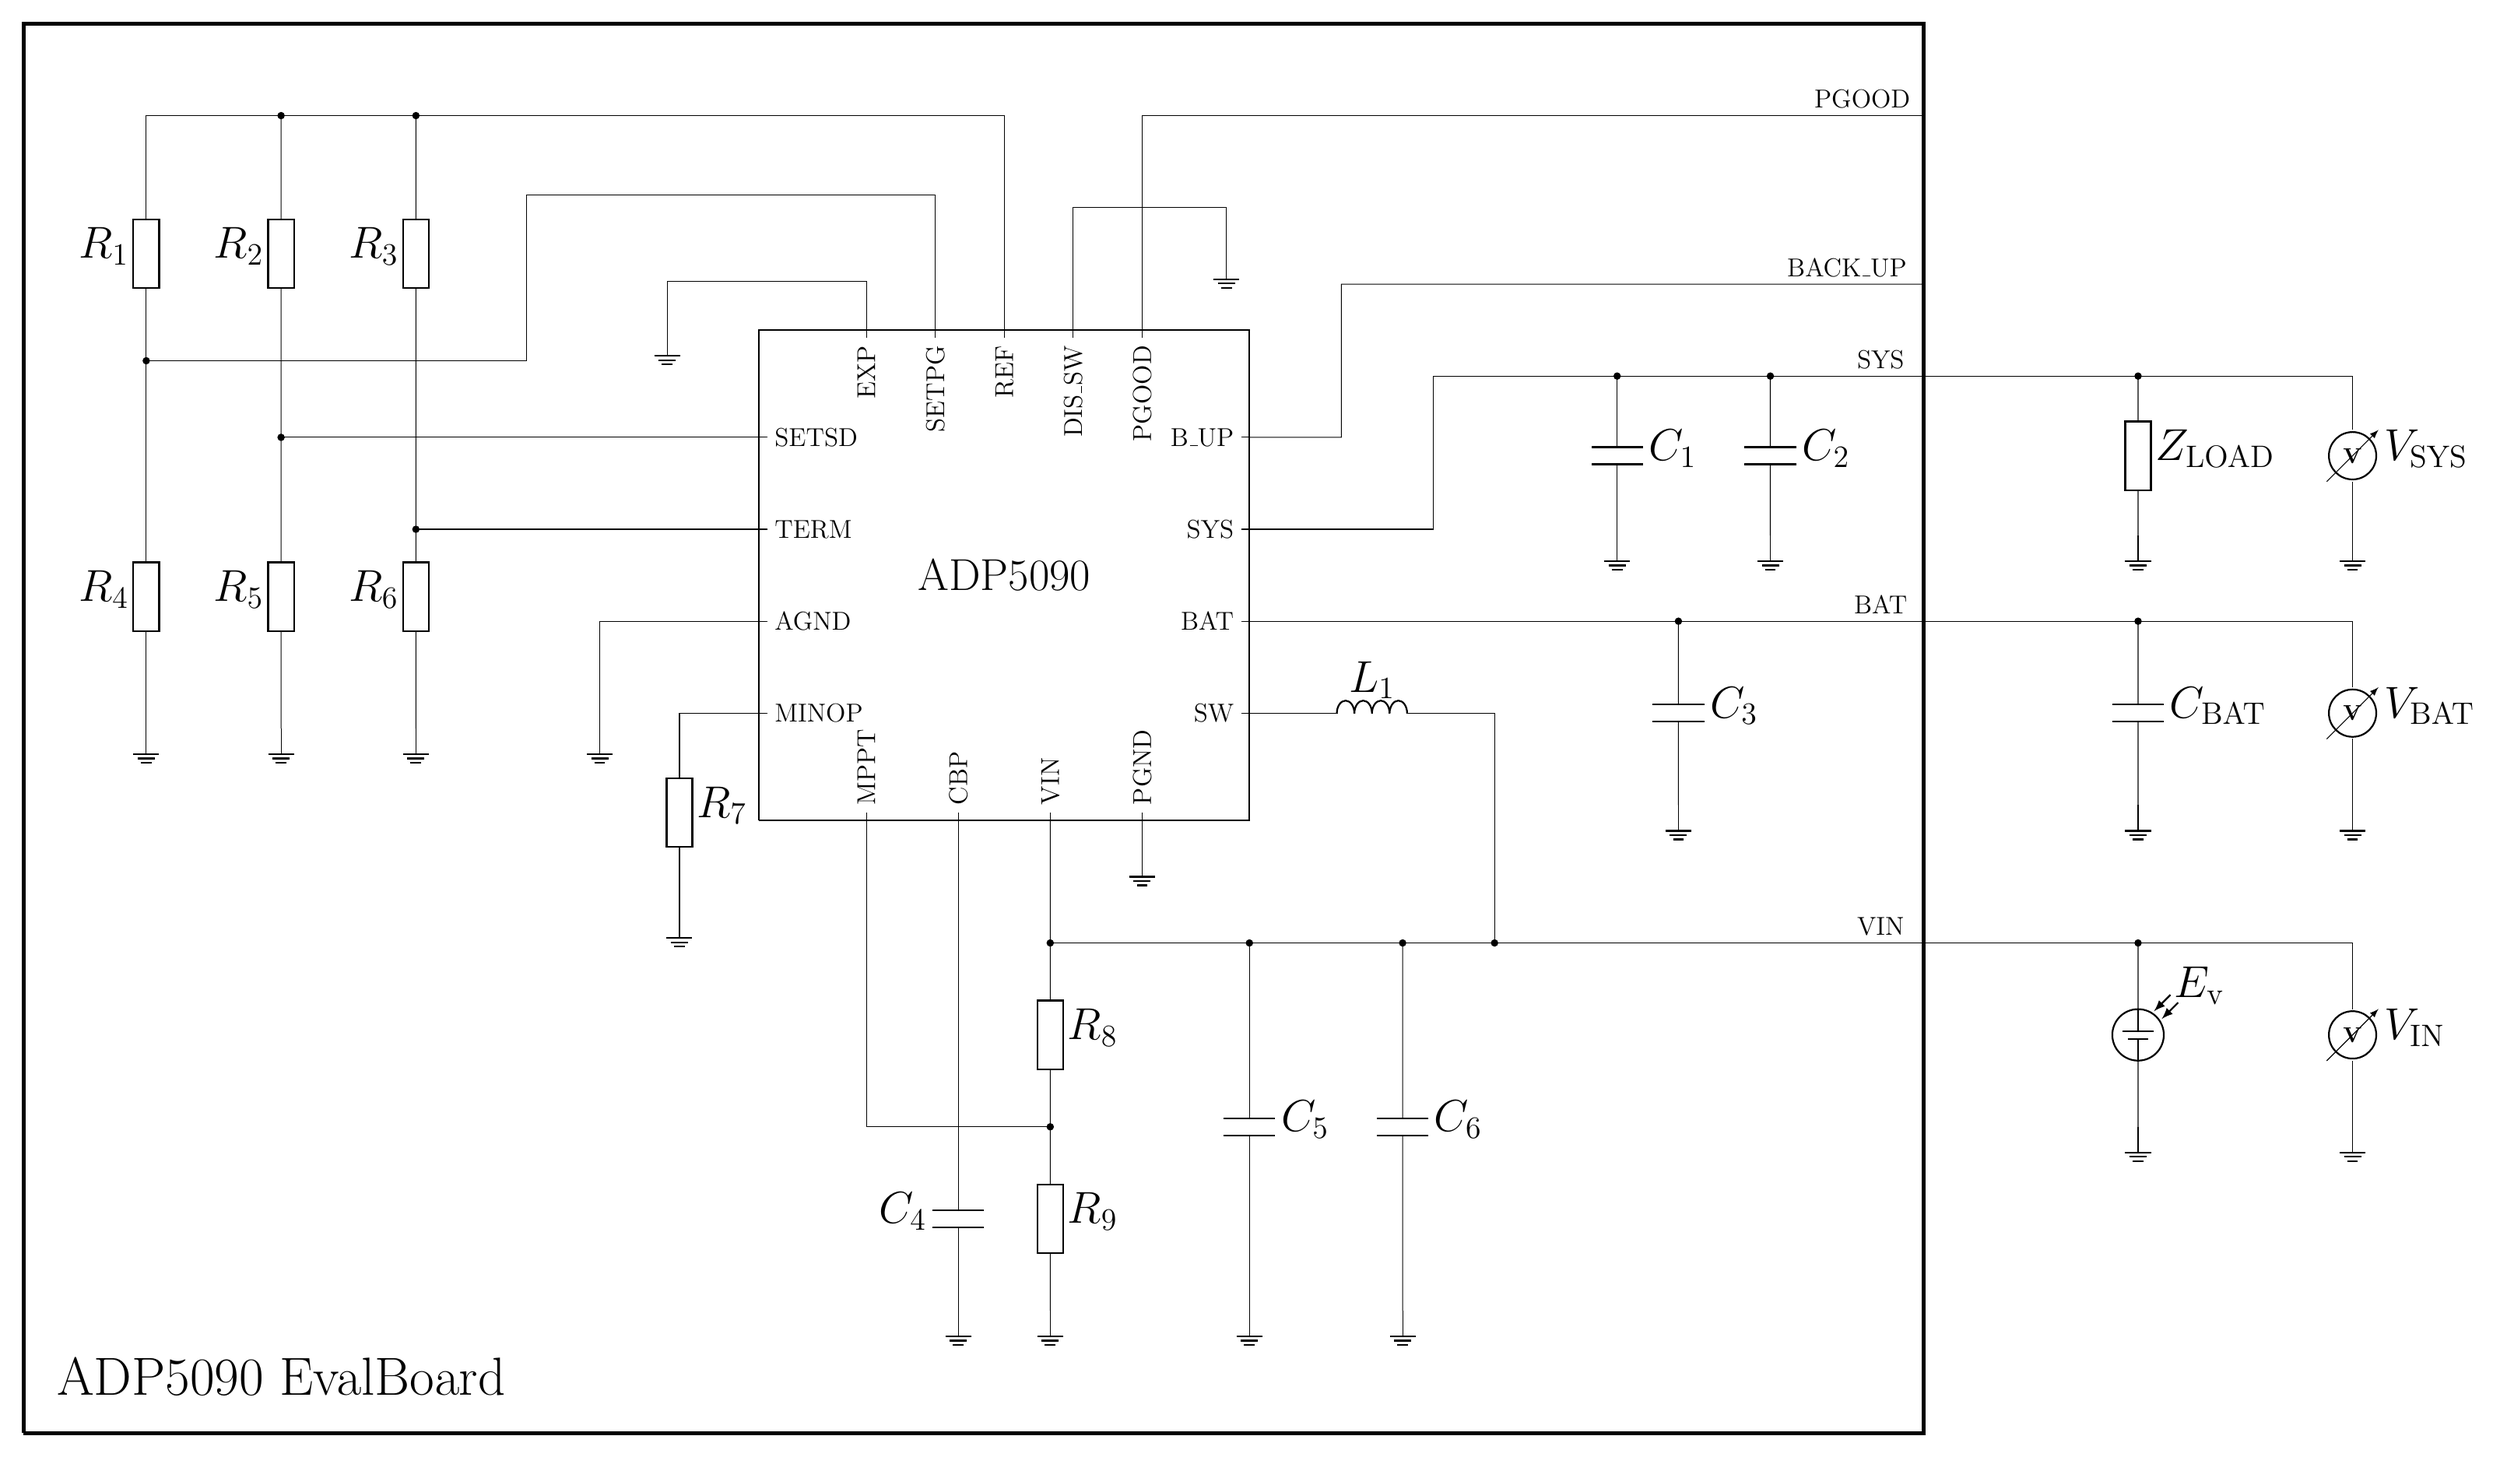
\begin{tikzpicture}
	%ADP
	\def\len{0.13}
	%Struktur
	\draw[thick] (0, 0) -- ++(8,0) -- ++(0,8) -- ++(-8,0) -- ++(0,-8);
	\node at (4, 4) {\huge ADP5090};
	
	\tikzset{fontscale/.style = {font=\Huge}};
	
	%nodes links
	\draw (0,1.75) -- ++(\len,0) node[right]{\large MINOP};
	\draw (0,1.75+1.5) -- ++(\len,0) node[right]{\large AGND};
	\draw (0,1.75+1.5*2) -- ++(\len,0) node[right]{\large TERM};
	\draw (0,1.75+1.5*3) -- ++(\len,0) node[right]{\large SETSD};
	%nodes oben
	\draw (1.75,8) --++(0,-\len) node[rotate=90, anchor=east]{\large EXP};
	\draw (1.75+1.125,8) --++(0,-\len) node[rotate=90, anchor=east]{\large SETPG};
	\draw (1.75+1.125*2,8) --++(0,-\len) node[rotate=90, anchor=east]{\large REF};
	\draw (1.75+1.125*3,8) --++(0,-\len) node[rotate=90, anchor=east]{\large DIS\_SW};
	\draw (1.75+1.125*4,8) --++(0,-\len) node[rotate=90, anchor=east]{\large PGOOD};
	%nodes rechts
	\draw (8, 1.75) --++(-\len,0) node[left]{\large SW};
	\draw (8, 1.75+1.5) --++(-\len,0) node[left]{\large BAT};
	\draw (8, 1.75+1.5*2) --++(-\len,0) node[left]{\large SYS};
	\draw (8, 1.75+1.5*3) --++(-\len,0) node[left]{\large B\_UP};
	%nodes unten
	\draw (1.75,0) --++ (0,\len) node[rotate=90, anchor=west]{\large MPPT};
	\draw (1.75+1.5,0) --++ (0,\len) node[rotate=90, anchor=west]{\large CBP};
	\draw (1.75+1.5*2,0) --++ (0,\len) node[rotate=90, anchor=west]{\large VIN};
	\draw (1.75+1.5*3,0) --++ (0,\len) node[rotate=90, anchor=west]{\large PGND};
		
	%Schaltung Evalboard
	\def\ps{1.5}
	
	\draw (1.75,8)--(1.75,8.8)--(-1.5,8.8) -- (-1.5,8) node[ground]{};
	\draw (1.75+1.125*3, 8) --++(0,2)--++(2.5,0)--++(0,-0.75) node[ground]{};
	\draw (0,1.75)--(-1.3,1.75) to[R=\huge $R_7$] (-1.3,-1.5) node[ground]{};
	\draw (0,3.25)--(-2.6,3.25)--(-2.6,1.5) node[ground]{};
	\draw (1.75+1.5*3, 0)--++(0,-0.5) node[ground]{};
			
	\draw (-10,1.5) node[ground]{} to[R=\huge $R_4$] (-10,5.8)--(-10, 7) to[R=\huge $R_1$] (-10,11.5)--(1.75+1.125*2,11.5)--++(0,-3.5);	
	\draw (-7.8,1.5) node[ground]{} to[R=\huge $R_5$] (-7.8,5.8)--(-7.8, 7) to[R=\huge $R_2$] (-7.8,11.5);
	\filldraw (-7.8,11.5) circle[radius=\ps pt];
	\draw (-5.6,1.5) node[ground]{} to[R=\huge $R_6$] (-5.6,5.8)--(-5.6, 7) to[R=\huge $R_3$] (-5.6,11.5);
	\filldraw (-5.6,11.5) circle[radius=\ps pt];
	\draw (0,1.75+1.5*2)--(-5.6,1.75+1.5*2);
	\filldraw (-5.6,1.75+1.5*2) circle[radius=\ps pt];
	\draw (0,1.75+1.5*3)--(-7.8,1.75+1.5*3);
	\filldraw (-7.8,1.75+1.5*3) circle[radius=\ps pt];	
	\filldraw (-10,7.5) circle[radius=\ps pt];	
	\draw (-10,7.5)--(-3.8,7.5)--(-3.8,10.2)--(1.75+1.125, 10.2)--(1.75+1.125,8);
	
	\draw (1.75+3, 0) --++(0,-2) to[R=\huge $R_8$] (1.75+3, -5) to[R=\huge $R_9$] (1.75+3, -8) node[ground]{};
	\draw (1.75+1.5, -8) node[ground]{} to[C=\huge $C_4$] (1.75+1.5,-5)--(1.75+1.5,0);	
	\filldraw (1.75+1.5*2, -5) circle[radius=\ps pt];
	\draw (1.75,0)--(1.75,-5)--(1.75+3,-5);
	\filldraw (1.75+1.5*2, -2) circle[radius=\ps pt];
	\draw (1.75+3,-2)--(19,-2);
	\filldraw (8, -2) circle[radius=\ps pt];
	\filldraw (10.5, -2) circle[radius=\ps pt];
	\draw (8,-2) to[C=\huge $C_5$] (8, -8) node[ground]{};
	\draw (10.5,-2) to[C=\huge $C_6$] (10.5, -8) node[ground]{};
	
	\draw (8,1.75) to[L=\huge $L_1$] (12,1.75)--(12,-2);
	\filldraw (12, -2) circle[radius=\ps pt];	
	\draw (8,1.75+1.5) -- (19, 1.75+1.5);
	\filldraw (15, 1.75+1.5) circle[radius=\ps pt];
	\draw (15, 1.75+1.5) to[C=\huge $C_3$] (15,0.25) node[ground]{};
	\draw (8, 1.75+4.5)--++(1.5,0)--++(0,2.5)--(19,1.75+4.5+2.5);
	\draw (8,1.75+3) -- ++(3,0)--++(0,2.5)--(19,1.75+5.5);
	\filldraw (14, 1.75+5.5) circle[radius=\ps pt];
	\filldraw (16.5, 1.75+5.5) circle[radius=\ps pt];
	\draw (14, 1.75+5.5) to[C=\huge $C_1$] ++(0,-2.6) node[ground]{};
	\draw (16.5, 1.75+5.5) to[C=\huge $C_2$] ++(0,-2.6) node[ground]{};
	\draw (1.75+1.125*4,8)--++(0,3.5)--(19,11.5);
	
	\node[above] at (18.3,-2){\large VIN};
	\node[above] at (18.3,1.75+1.5){\large BAT};
	\node[above] at (18.3,1.75+3+2.5){\large SYS};
	\node[above] at (17.75,1.75+4.5+2.5){\large BACK\_UP};
	\node[above] at (18,11.5){\large PGOOD};
	
	%umranden
	\draw[line width=2pt] (-12,-10)--(19,-10)--(19,13)--(-12,13)--(-12,-10);
	\node[above] at (-7.8,-9.5) {\Huge ADP5090 EvalBoard};

	%Schaltung rundherum
	%eigenes Voltmeter
	\newcommand{\mymeter}[2]
	{
		\begin{scope}[transform shape, rotate=#2]
		\draw[thick] (#1)node(){$\mathbf{V}$} circle (11pt);
		\draw[rotate=45,-latex] (#1) +(-17pt,0) -- +(17pt,0);
		\end{scope}	
	};
	\draw (19, -2) --(26,-2) to[voltmeter, color=white, name=M, label=\huge $V_{\mathrm{IN}}$] (26,-5) node[ground]{};
	\mymeter{M}{0};
	\filldraw (22.5, -2) circle[radius=\ps pt];
	\draw (22.5,-5) node[ground]{} to[pvsource] (22.5,-2);
		
	\draw (19, 3.25)--(26,3.25) to[voltmeter, color=white, name=M, label=\huge $V_{\mathrm{BAT}}$] (26,3.25-3) node[ground]{};
	\mymeter{M}{0};	
	\filldraw (22.5, 3.25) circle[radius=\ps pt];
	\draw (22.5, 3.25) to[C=\huge $C_{\mathrm{BAT}}$] (22.5, 3.25-3) node[ground]{};
	
	\draw (19, 7.25)--(26,7.25) to[voltmeter, color=white, name=M, label=\huge $V_{\mathrm{SYS}}$] (26,7.25-2.6) node[ground]{};
	\mymeter{M}{0}
	\filldraw (22.5, 7.25) circle[radius=\ps pt];
	\draw (22.5,7.25) to[R=\huge $Z_{\mathrm{LOAD}}$] (22.5,7.25-2.6) node[ground]{};
	\node at (23.5,-2.7) {\huge $E_\mathrm{v}$};	
		
	%bel=$V_{\mathrm{BAT}}$] (0,3) -- (4,3);
	%\mymeter{M}{0}
	%\draw (2,0) node[ground]{} to[C] (2,3);
	
	%\draw (0,5) node[ground]{} to[voltmeter, color=white, name=M, label=$V_{\mathrm{IN}}$] (0,8) -- (4,8);
	%\mymeter{M}{0}
	%\draw (2,5) node[ground]{} to[pvsource] (2,8);
	
	%ADP
	%\draw[thick] (4,2) -- ++(5,0) -- ++(0,7) -- ++(-5,0) -- ++(0,-7);		
\end{tikzpicture}
\end{document}